\documentclass[aspectratio=169, xcolor=dvipsnames]{beamer}

% --- Theme Setup ---
\usetheme{Madrid}
\usecolortheme{default}

% --- Packages ---
\usepackage{graphicx}
\usepackage{xcolor}
\usepackage{booktabs}
\usepackage{hyperref}
\usepackage{adjustbox}
\usepackage{amssymb}
\usepackage{amsmath}
\usepackage{listings}
\usepackage{caption}
\usepackage{tikz}

\lstset{
  basicstyle=\ttfamily\small,
  keywordstyle=\color{blue}\bfseries,
  stringstyle=\color{red},
  showstringspaces=false,
  breaklines=true
}

% --- Title Information ---
\title{Module 21}
\subtitle{Relational Database Design/1}
\author{Milav Dabgar}
\institute{www.milav.in}
\date{\today}

\begin{document}

% Title Slide
\begin{frame}
    \titlepage
\end{frame}

\begin{frame}{Week Recap}
    \begin{itemize}[<+->]
        \item Discussed relational algebra with examples
        \item Introduced tuple relational and domain relational calculus
        \item Illustrated equivalence of algebra and calculus
        \item Introduced the Design Process for Database Systems
        \item Elucidated the E-R Model for real world representation with entities, entity sets, attributes, and relationships
        \item Illustrated ER Diagram notation for ER Models
        \item Discussed translation of ER Models to Relational Schema and extended features of ER Model
        \item Deliberated on various design issues
    \end{itemize}
\end{frame}

\begin{frame}{Module Objectives}
    \begin{block}{Goals}
        \begin{itemize}[<+->]
            \item To identify the features of good relational design
            \item To familiarize with the First Normal Form
        \end{itemize}
    \end{block}
\end{frame}

\begin{frame}{Module Outline}
    \begin{itemize}[<+->]
        \item Features of Good Relational Design
        \item Atomic Domains and First Normal Form
    \end{itemize}
\end{frame}

\section{Features of Good Relational Design}
\begin{frame}
  \vfill
  \centering
  \begin{beamercolorbox}[sep=8pt,center,shadow=true,rounded=true]{title}
    \usebeamerfont{title}Features of Good Relational Design\par%
  \end{beamercolorbox}
  \vfill
\end{frame}

\begin{frame}{Good Relational Design}
    \begin{itemize}[<+->]
        \item Reflects real-world structure of the problem
        \item Can represent all expected data over time
        \item Avoids redundant storage of data items
        \item Provides efficient access to data
        \item Supports the maintenance of data integrity over time
        \item Clean, consistent, and easy to understand
        \item Note: These objectives are sometimes contradictory!
    \end{itemize}
\end{frame}

\begin{frame}{What is a Good Schema?}
    \textbf{instructor with department}
    \begin{center}
    \resizebox{\textwidth}{!}{
    \begin{tabular}{|l|l|l|l|l|l|}
    \hline
    \textbf{ID} & \textbf{name} & \textbf{salary} & \textbf{dept\_name} & \textbf{building} & \textbf{budget} \\ \hline
    22222 & Einstein & 95000 & Physics & Watson & 70000 \\ 
    12121 & Wu & 90000 & Finance & Painter & 120000 \\ 
    32343 & El Said & 60000 & History & Painter & 50000 \\ 
    45565 & Katz & 75000 & Comp. Sci. & Taylor & 100000 \\ 
    98345 & Kim & 80000 & Elec. Eng. & Taylor & 85000 \\ 
    76766 & Crick & 72000 & Biology & Watson & 90000 \\ 
    10101 & Srinivasan & 65000 & Comp. Sci. & Taylor & 100000 \\ 
    58583 & Califieri & 62000 & History & Painter & 50000 \\ 
    83821 & Brandt & 92000 & Comp. Sci. & Taylor & 100000 \\ 
    15151 & Mozart & 40000 & Music & Packard & 80000 \\ 
    33456 & Gold & 87000 & Physics & Watson & 70000 \\ 
    76543 & Singh & 80000 & Finance & Painter & 120000 \\ \hline
    \end{tabular}
    }
    \end{center}
    \begin{itemize}[<+->]
        \item ID : Key
        \item building, budget : Redundant Information
        \item name, salary, dept\_name : No Redundant Information
    \end{itemize}
\end{frame}

\begin{frame}{What is a Good Schema? (Cont.)}
    \textbf{instructor}
    \begin{center}
    \begin{tabular}{|l|l|l|l|}
    \hline
    \textbf{ID} & \textbf{name} & \textbf{dept\_name} & \textbf{salary} \\ \hline
    10101 & Srinivasan & Comp. Sci. & 65000 \\ 
    12121 & Wu & Finance & 90000 \\ 
    15151 & Mozart & Music & 40000 \\ 
    22222 & Einstein & Physics & 95000 \\ 
    32343 & El Said & History & 60000 \\ 
    33456 & Gold & Physics & 87000 \\ 
    45565 & Katz & Comp. Sci. & 75000 \\ 
    58583 & Califieri & History & 62000 \\ 
    76543 & Singh & Finance & 80000 \\ 
    76766 & Crick & Biology & 72000 \\ 
    83821 & Brandt & Comp. Sci. & 92000 \\ 
    98345 & Kim & Elec. Eng. & 80000 \\ \hline
    \end{tabular}
    \end{center}
\end{frame}

\begin{frame}{What is a Good Schema? (Cont.)}
    \textbf{department}
    \begin{center}
    \begin{tabular}{|l|l|l|}
    \hline
    \textbf{dept\_name} & \textbf{building} & \textbf{budget} \\ \hline
    Biology & Watson & 90000 \\ 
    Comp. Sci. & Taylor & 100000 \\ 
    Elec. Eng. & Taylor & 85000 \\ 
    Finance & Painter & 120000 \\ 
    History & Painter & 50000 \\ 
    Music & Packard & 80000 \\ 
    Physics & Watson & 70000 \\ \hline
    \end{tabular}
    \end{center}
\end{frame}

\begin{frame}{What is a Good Schema? (2)}
    \begin{center}
        % Missing image removed
    \end{center}
    \begin{itemize}[<+->]
        \item Consider combining relations
        \item \texttt{sec\_class(sec\_id, building, room\_number)} and
        \item \texttt{section(course\_id, sec\_id, semester, year)}
        \item into one relation
        \item \texttt{section(course\_id, sec\_id, semester, year, building, room\_number)}
        \item No repetition in this case
    \end{itemize}
\end{frame}

\section{Redundancy and Anomaly}
\begin{frame}
  \vfill
  \centering
  \begin{beamercolorbox}[sep=8pt,center,shadow=true,rounded=true]{title}
    \usebeamerfont{title}Redundancy and Anomaly\par%
  \end{beamercolorbox}
  \vfill
\end{frame}

\begin{frame}{Redundancy and Anomaly}
    \begin{itemize}[<+->]
        \item \textbf{Redundancy}: having multiple copies of same data in the database.
        \item This problem arises when a database is not normalized
        \item It leads to anomalies
        \item \textbf{Anomaly}: inconsistencies that can arise due to data changes in a database with insertion, deletion, and update
        \item These problems occur in poorly planned, un-normalised databases where all the data is stored in one table (a flat-file database)
    \end{itemize}
    \vspace{1em}
    \uncover<6->{There can be three kinds of anomalies:}
    \begin{itemize}[<+->]
        \item Insertions Anomaly
        \item Deletion Anomaly
        \item Update Anomaly
    \end{itemize}
\end{frame}

\begin{frame}{Redundancy and Anomaly (2)}
    \begin{itemize}[<+->]
        \item \textbf{Insertions Anomaly}
        \begin{itemize}
            \item[$\triangleright$] When the insertion of a data record is not possible without adding some additional unrelated data to the record
            \item[$\triangleright$] We cannot add an Instructor in \texttt{instructor\_with\_department} if the department does not have a building or budget
        \end{itemize}
        \item \textbf{Deletion Anomaly}
        \begin{itemize}
            \item[$\triangleright$] When deletion of a data record results in losing some unrelated information that was stored as part of the record that was deleted from a table
            \item[$\triangleright$] We delete the last Instructor of a Department from \texttt{instructor\_with\_department}, we lose building and budget information
        \end{itemize}
        \item \textbf{Update Anomaly}
        \begin{itemize}
            \item[$\triangleright$] When a data is changed, which could involve many records having to be changed, leading to the possibility of some changes being made incorrectly
            \item[$\triangleright$] When the budget changes for a Department having a large number of Instructors in \texttt{instructor\_with\_department}, application may miss some of them
        \end{itemize}
    \end{itemize}
\end{frame}

\begin{frame}{Redundancy and Anomaly (3)}
    \begin{itemize}[<+->]
        \item We have observed the following:
        \item \textbf{Redundancy $\Rightarrow$ Anomaly}
        \item Relations \texttt{instructor} and \texttt{department} is better than \texttt{instructor\_with\_department}
        \item What causes redundancy?
        \item \textbf{Dependency $\Rightarrow$ Redundancy}
        \item \texttt{dept\_name} uniquely decides building and budget. A department cannot have two different budgets or buildings. So building and budget depends on \texttt{dept\_name}
        \item How to remove, or at least minimize, redundancy?
        \item Decompose (partition) the relation into smaller relations
        \item \texttt{instructor\_with\_department} can be decomposed into \texttt{instructor} and \texttt{department}
        \item \textbf{Good Decomposition $\Rightarrow$ Minimization of Dependency}
        \item Is every decomposition good?
        \item No. It needs to preserve information, honour the dependencies, be efficient etc.
        \item Various schemes of normalization ensure good decomposition
        \item \textbf{Normalization $\Rightarrow$ Good Decomposition}
    \end{itemize}
\end{frame}

\section{Decomposition}
\begin{frame}
  \vfill
  \centering
  \begin{beamercolorbox}[sep=8pt,center,shadow=true,rounded=true]{title}
    \usebeamerfont{title}Decomposition\par%
  \end{beamercolorbox}
  \vfill
\end{frame}

\begin{frame}{Decomposition}
    \begin{itemize}[<+->]
        \item Suppose we had started with \texttt{inst\_dept}. How would we know to split up (decompose) it into \texttt{instructor} and \texttt{department}?
        \item Write a rule `if there were a schema (\texttt{dept\_name}, \texttt{building}, \texttt{budget}), then \texttt{dept\_name} would be a candidate key'
        \item Denote as a functional dependency: \texttt{dept\_name} $\rightarrow$ \texttt{building}, \texttt{budget}
        \item In \texttt{inst\_dept}, because \texttt{dept\_name} is not a candidate key, the building and budget of a department may have to be repeated.
        \item This indicates the need to decompose \texttt{inst\_dept}
    \end{itemize}
\end{frame}

\begin{frame}{Decomposition (2)}
    \begin{itemize}[<+->]
        \item Not all decompositions are good
        \item Suppose we decompose 
        \item \texttt{employee(ID, name, street, city, salary)} into \texttt{employee1(ID, name)} and \texttt{employee2(name, street, city, salary)}
        \item Note that if \texttt{name} can be duplicate, then \texttt{employee2} is a weak entity set and cannot exist without an identifying relationship
        \item Consequently, this decomposition cannot preserve the information
        \item The next slide shows how we lose information - we cannot reconstruct the original \texttt{employee} relation - and so, this is a \textbf{lossy decomposition}.
    \end{itemize}
\end{frame}

\begin{frame}{Decomposition (3): Lossy Decomposition}
    \begin{center}
        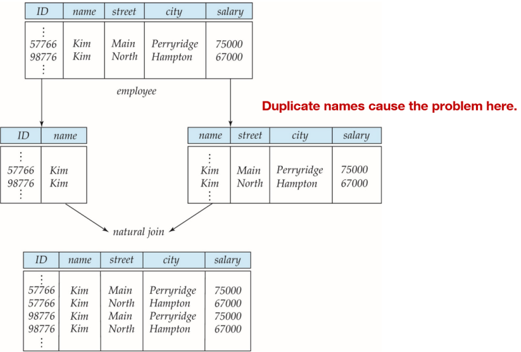
\includegraphics[width=0.9\textwidth,height=0.7\textheight,keepaspectratio]{../Lecture 5.1_artifacts/image_000017_263bde584a83f092972d014f681d0d093ee699d4656e7e56c7ea2ea7c135d3c5.png}
    \end{center}
\end{frame}

\begin{frame}{Decomposition (4): Lossless-Join Decomposition}
    \begin{itemize}[<+->]
        \item Lossless Join Decomposition
        \item Decomposition of $R = (A, B, C)$ into $R_1 = (A, B)$, $R_2 = (B, C)$
    \end{itemize}
    \begin{center}
        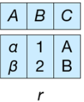
\includegraphics[width=0.45\textwidth,height=0.4\textheight,keepaspectratio]{../Lecture 5.1_artifacts/image_000019_46c3bf1c946639025550d24f4193f71ce74f3836dbb3b5831e918d82cc13d6f8.png}
        \hfill
        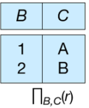
\includegraphics[width=0.45\textwidth,height=0.4\textheight,keepaspectratio]{../Lecture 5.1_artifacts/image_000021_35129a9291b930ad6c5f3504cfd336af1f9dceeb832737a8553538d22e12cd62.png}
    \end{center}
\end{frame}

\begin{frame}{Decomposition (5): Lossless-Join Decomposition}
    \begin{block}{Definition}
        \begin{itemize}[<+->]
            \item Lossless Join Decomposition is a decomposition of a relation $R$ into relations $R_1, R_2$ such that if we perform natural join of two smaller relations it will return the original relation
        \end{itemize}
        \[ R_1 \cup R_2 = R, \quad R_1 \cap R_2 \neq \phi \]
        \[ \forall r \in R, \quad r_1 = \Pi_{R_1}(r), \quad r_2 = \Pi_{R_2}(r) \]
        \[ r_1 \bowtie r_2 = r \]
    \end{block}
    \begin{itemize}[<+->]
        \item This is effective in removing redundancy from databases while preserving the original data
        \item In other words by lossless decomposition it becomes feasible to reconstruct the relation $R$ from decomposed tables $R_1$ and $R_2$ by using Joins
    \end{itemize}
\end{frame}

\section{Atomic Domains and First Normal Form}
\begin{frame}
  \vfill
  \centering
  \begin{beamercolorbox}[sep=8pt,center,shadow=true,rounded=true]{title}
    \usebeamerfont{title}Atomic Domains and First Normal Form\par%
  \end{beamercolorbox}
  \vfill
\end{frame}

\begin{frame}{First Normal Form (1NF)}
    \begin{itemize}[<+->]
        \item A domain is atomic if its elements are considered to be indivisible units
        \item Examples of non-atomic domains:
        \begin{itemize}
            \item[$\triangleright$] Set of names, composite attributes
            \item[$\triangleright$] Identification numbers like CS101 that can be broken up into parts
        \end{itemize}
    \end{itemize}
    \uncover<4->{
    \begin{block}{Definition of 1NF}
        A relational schema R is in First Normal Form (1NF) if:
        \begin{itemize}
            \item the domains of all attributes of R are atomic
            \item the value of each attribute contains only a single value from that domain
        \end{itemize}
    \end{block}
    }
    \begin{itemize}[<+(4)->]
        \item Non-atomic values complicate storage and encourage redundant (repeated) storage of data
        \item Example: Set of accounts stored with each customer, and set of owners stored with each account
        \item We assume all relations are in first normal form
    \end{itemize}
\end{frame}

\begin{frame}{First Normal Form (2)}
    \begin{itemize}[<+->]
        \item Atomicity is actually a property of how the elements of the domain are used
        \item Strings would normally be considered indivisible
        \item Suppose that students are given roll numbers which are strings of the form CS0012 or EE1127
        \item If the first two characters are extracted to find the department, the domain of roll numbers is not atomic
        \item Doing so is a bad idea
        \begin{itemize}
            \item[$\triangleright$] Leads to encoding of information in application program rather than in the database
        \end{itemize}
    \end{itemize}
\end{frame}

\begin{frame}{First Normal Form (3)}
    \begin{itemize}
        \item The following is not in 1NF
    \end{itemize}
    \textbf{customer}
    \begin{center}
    \begin{tabular}{|l|l|l|l|}
    \hline
    \textbf{Customer ID} & \textbf{First Name} & \textbf{Surname} & \textbf{Telephone Number} \\ \hline
    123 & Pooja & Singh & 555-861-2025, 192-122-1111 \\ 
    456 & San & Zhang & (555) 403-1659 Ext. 53, 182-929-2929 \\ 
    789 & John & Doe & 555-808-9633 \\ \hline
    \end{tabular}
    \end{center}
    \begin{itemize}[<+->]
        \item A telephone number is composite
        \item Telephone number is multi-valued
    \end{itemize}
\end{frame}

\begin{frame}{First Normal Form (4)}
    \begin{itemize}
        \item Consider:
    \end{itemize}
    \textbf{customer}
    \begin{center}
    \begin{tabular}{|l|l|l|l|l|}
    \hline
    \textbf{Customer ID} & \textbf{First Name} & \textbf{Surname} & \textbf{Telephone Number1} & \textbf{Telephone Number2} \\ \hline
    123 & Pooja & Singh & 555-861-2025 & 192-122-1111 \\ 
    456 & San & Zhang & (555) 403-1659 Ext. 53 & 182-929-2929 \\ 
    789 & John & Doe & 555-808-9633 & \\ \hline
    \end{tabular}
    \end{center}
    \begin{itemize}[<+->]
        \item is in 1NF if telephone number is not considered composite
        \item However, conceptually, we have two attributes for the same concept
        \begin{itemize}
            \item[$\triangleright$] Arbitrary and meaningless ordering of attributes
            \item[$\triangleright$] How to search telephone numbers
            \item[$\triangleright$] Why only two numbers?
        \end{itemize}
    \end{itemize}
\end{frame}

\begin{frame}{First Normal Form (5)}
    \begin{itemize}[<+->]
        \item Is the following in 1NF?
        \item Duplicated information
        \item ID is no more the key. Key is (ID, Telephone Number)
    \end{itemize}
    \textbf{customer}
    \begin{center}
    \begin{tabular}{|l|l|l|l|}
    \hline
    \textbf{Customer ID} & \textbf{First Name} & \textbf{Surname} & \textbf{Telephone Number} \\ \hline
    123 & Pooja & Singh & 555-861-2025 \\ 
    123 & Pooja & Singh & 192-122-1111 \\ 
    456 & San & Zhang & 182-929-2929 \\ 
    456 & San & Zhang & (555) 403-1659 Ext. 53 \\ 
    789 & John & Doe & 555-808-9633 \\ \hline
    \end{tabular}
    \end{center}
\end{frame}

\begin{frame}{First Normal Form (6)}
    \begin{itemize}[<+->]
        \item Better to have 2 relations:
        \item One-to-Many relationship between parent and child relations
        \item Incidentally, satisfies 2NF and 3NF
        \item Decomposition helps to attain 1NF for the embedded one-to-many relationship
    \end{itemize}
    \begin{center}
        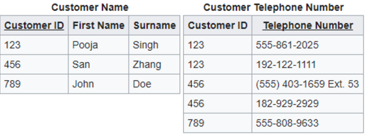
\includegraphics[width=0.9\textwidth,height=0.4\textheight,keepaspectratio]{../Lecture 5.1_artifacts/image_000031_b1c6d6a0156bbbe24c1ed872a8ca273c539ba586de33ca6de8055ecf7e3a3b63.png}
    \end{center}
\end{frame}

\begin{frame}{Module Summary}
    \begin{block}{Summary}
        \begin{itemize}[<+->]
            \item Identified the features of good relational design
            \item Familiarized with the First Normal Form
        \end{itemize}
    \end{block}
    \vspace{2em}
    \begin{center}
    \small \textit{Slides used in this presentation are borrowed from \url{http://db-book.com/} with kind permission of the authors.} \\
    \small \textit{Edited and new slides are marked with 'PPD'.}
    \end{center}
\end{frame}

\end{document}
